The blockchain technology is first proposed in Satoshi Nakamoto’s paper, Bitcoin: A Peer-to-Peer Electronic Cash System \cite{Nakamoto2008}, in 2008. It created a new type of digital currency, called cryptocurrency. For example, Bitcoin \cite{bitcoin} and Ethereum \cite{ethereum} are two of the well-known cryptocurrency. Cryptocurrency has a significant characteristic that distinguishes it from other currency: it is decentralized. This means that there is no authority in cryptocurrency. Therefore, it is important to guarantee the validity of transactions, and it is fulfilled by consensus protocols which use cryptography techniques. \cite{Narayanan2016}

The major process of the consensus protocol starts with the creation of a transaction. This transaction is distributed over the blockchain network. In this state, the transaction is not-mined and therefore not persistent. Every node in the network has their own transaction pools that contain the not-mined transactions.

In a blockchain system with the proof-of-work protocol, the nodes maintain the blockchain data structure by themselves. They compete against each other in extending the blockchain by creating new blocks that persistently store transactions from the transaction pools. The addition of new blocks provides effort, since it is necessary to solve a cryptographic puzzle with the characteristic that it is hard to solve, but easy to verify given a correct solution. The solving process is called mining. A correct solution is distributed over the network and verified by the remaining network participants. In the case that the verification succeeds, the block is added to the blockchain, and the containing transactions are removed from the transaction pools.

\section{Motivation}

There are two factors that play important roles in the mining processes: the network delay on the blockchain network and the mining strategy of miners. Transactions are published through the blockchain network, but each node receives them at a different time due to the unstable network. Therefore, each miner has different pending transactions in their own transaction pools. Moreover, each miner mines a block according to their own mining strategies simultaneously. The blocks generated by miners are different from each other, and they are also published through the unstable network. Consequently, it is possible that the set of nodes partitions into different groups that work on different instances of the blockchain. These blockchains are maintained simultaneously until one blockchain becomes longer. The longest blockchain in the network is assumed to be the correct one, which is resolved by the consensus protocol.

In a real blockchain system, for example, there are about ten thousand of nodes in Bitcoin in April 2018. For such wide and massive blockchain networks, it is hard to analyze the individual behavior of each node, e.g., the influences of the mining strategy to the mining processes under the unstable peer-to-peer network. Moreover, the mining processes of a blockchain system described earlier are dynamic and complex. Therefore, to focus on the research of mining processes in a blockchain system, we decide to provide a visualization tool to display the influences of network delay and the mining strategies on mining processes step by step.

\section{Methodology}

In Figure \ref{fig:the method}, it explains the basic idea of the solution. A simulation of the blockchain system is based on a multi-agent system, and a watchdog monitors and records the mining activities in the blockchain system. Thus, when the transactions and blocks are published and received, the watchdog sends the required data to a visualizer, which is responsible for visualizing all the mining events that happened in the blockchain system. 

\begin{figure}[htb]
    \centering
    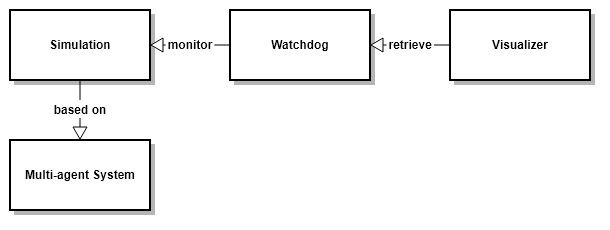
\includegraphics[width=\textwidth]{intro_method}
    \caption{The method.}
    \label{fig:the method}
\end{figure}

The application is able to visualize the steps of mining processes of each node in real-time. By setting the parameters of network delay and the mining strategy, researchers can analyze and observe the mining processes with predefined conditions in the blockchain system. Additionally, in order to replay the same result of blockchain processes, it is possible to provide a configuration file that defines all the properties of nodes and parameters of network delay and the mining strategy in the blockchain system.

\section{Contribution}

There are 8 online visualization applications that are summarized by Tri A. Sundara et al. \cite{Sundara2017}. However, these visualization applications only display the static information in Bitcoin network, and they can not statisfy the goal which helps users to understanding the dynamic mining processes. Additionally, there are several previous literature that provide visualization tools \cite{Battista2015, Kuzuno2017, McGinn2016, Saublet2015, Fleder2015, Baumann2014} to analyze the patterns of transactions on Bitcoin network. These visualization tools are implemented for analysis, though our solution focuses on visualizing the actual mining processes. Amitai Porat et al. \cite{Porat} proposed a method to analyze the potential applications of proof-of-work based blockchain networks. They considered the influences of network latency to the blockchain system. Nevertheless, our solution also considered the influences of the mining strategy which are not presented in their work.

Comparing to other visualization tools for blockchain systems, our solution provides a clear visualization for the dynamic mining processes. Moreover, the mining processes are visualized step by step while the miners are publishing blocks through the network. Consequently, our solution is suitable for researching and understanding the complex mining processes with the factors of network delay and the mining strategy.

\section{Thesis Structure}

This thesis is composed of the following chapters.

\begin{itemize}
    \item \textbf{Chatper 2} \\
        The review of the previous literature is provided in this chapter, and the contribution of our approach.
    \item \textbf{Chatper 3} \\
        The assumptions and definitions of the blockchain system that is used in the visualization are given in this chapter.
    \item \textbf{Chatper 4} \\
        This chapter contains the architecture of the visualization application and the components that are implemented.
    \item \textbf{Chatper 5} \\
        In this chapter, the introduction to the usage of the visualization application is provided.
    \item \textbf{Chatper 6} \\
        Three scenarios that can be achieved by the visualization application are proposed in this chapter.
    \item \textbf{Chatper 7} \\
        At the end of this paper, the conclusion and the future work are discussed.
\end{itemize}
